\documentclass{beamer}
\usetheme{Warsaw}
\setbeamertemplate{headline}{}

\usepackage{ae,lmodern}
\usepackage[english]{babel}
\usepackage[utf8]{inputenc}
\usepackage[T1]{fontenc}

\usepackage{caption}
\captionsetup[figure]{labelformat=empty}

\PassOptionsToPackage{usenames,dvipsnames}{xcolor}
\usepackage{xcolor,colortbl}
\definecolor{DarkGrey}{HTML}{222222}
\definecolor{DarkBlue}{HTML}{004BA9}
\definecolor{DarkRed}{HTML}{CC1111}
\definecolor{DarkGreen}{HTML}{117711}
\definecolor{DarkOrange}{HTML}{CC7000}
\definecolor{LightGrey}{HTML}{DDDDDD}
\definecolor{LightBlue}{HTML}{F0F8FF}
\definecolor{codegreen}{rgb}{0,0.6,0}
\definecolor{codepurple}{rgb}{0.58,0,0.82}

\usepackage[cache=false]{minted}
\setminted[bash]{
   bgcolor=LightBlue,
   breaklines, breakanywhere,
   frame=single,
   autogobble
}
\usemintedstyle[python]{native}
\setminted[python]{
   bgcolor=black,
   breaklines, breakanywhere,
   autogobble
}

\usepackage{listings}
\usepackage{lstautogobble}
\lstdefinestyle{bash}{
    backgroundcolor=\color{DarkGrey},   
    commentstyle=\color{codegreen},
    keywordstyle=\color{magenta},
    numberstyle=\tiny\color{DarkGrey},
    stringstyle=\color{codepurple},
    basicstyle=\ttfamily\tiny\color{LightGrey},
    escapeinside={\%*}{*)},
    breakatwhitespace=false,         
    breaklines=true,                 
    captionpos=b,                    
    keepspaces=true,                 
    numbers=left,                    
    numbersep=5pt,                  
    showspaces=false,                
    showstringspaces=false,
    showtabs=false,
    showlines=false,
    tabsize=2
}

\usepackage{tikz}
\usetikzlibrary{calc,decorations.pathreplacing,arrows,arrows.meta,shapes,patterns, positioning}
\newcommand\BigLength{14.6em}
\newcommand\Height{2em}
\newcommand\Sep{0.6em}
\newcommand\Center{\BigLength*1/2}
\newcommand\BigBox{\BigLength+\Sep}
\newcommand\HalfBox{\BigLength*1/2-\Sep*1/4}
\newcommand\HalfLength{\BigLength*1/2-\Sep*5/4}
\newcommand\CenterL{\BigLength*1/4-\Sep*1/8}
\newcommand\CenterR{\BigLength*3/4+\Sep*1/8}
\tikzstyle{layer}=[rectangle,thick,text centered,
                     minimum height=\Height,minimum width=\BigLength]
\tikzstyle{short}=[rectangle,thick,text centered,
                     minimum height=\Height,minimum width=\HalfLength]
\tikzstyle{dibox}=[rectangle,thick,semitransparent,
                     minimum height=(\Height+\Sep)*2,minimum width=\BigBox]
\tikzstyle{vmbox}=[rectangle,thick,semitransparent,
                     minimum height=(\Height+\Sep)*3,minimum width=\HalfBox]
\tikzstyle{ctbox}=[rectangle,thick,semitransparent,
                     minimum height=(\Height+\Sep)*2,minimum width=\HalfBox]
\tikzstyle{vebox}=[rectangle,thick,semitransparent,
                     minimum height=(\Height+\Sep)*1,minimum width=\HalfBox]

\usepackage{hyperref}
\usepackage{grffile}


\AtBeginSection[]
{
   \begin{frame}
      \tableofcontents[currentsection]
   \end{frame}
}

\AtBeginSubsection[]
{
   \begin{frame}
      \tableofcontents[currentsection, currentsubsection, sectionstyle=shaded]
   \end{frame}
}

%----------------------------------------------------------------------------------------
\title{Introduction to Data Science}
\subtitle{with Python}
%----------------------------------------------------------------------------------------
\author{Alexis Bogroff}
\date{\today}



\begin{document}

\begin{frame}
   \titlepage
\end{frame}

\begin{frame}
   \tableofcontents
\end{frame}

\section{Linux}
\section{Git}
\section{Python}

%----------------------------------------------------------------------------------------
\subsection{Python and Linux Similarities}
%----------------------------------------------------------------------------------------

\begin{frame}\frametitle{OS}
   \centering
   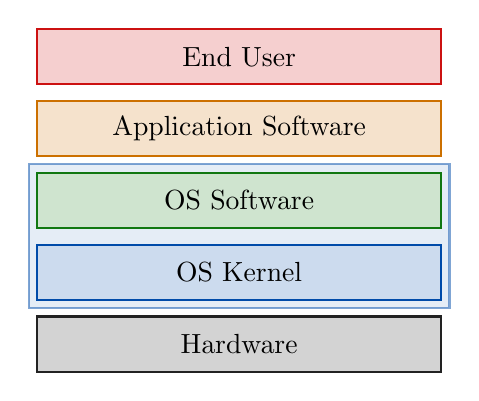
\begin{tikzpicture}[scale=1]
      \node[layer] at (\Center,\Height*1/2+\Sep*0) [draw=DarkGrey,fill=DarkGrey!20] {Hardware};
      \node[dibox] at (\Center,\Height*2+\Sep*3/2) [draw=DarkBlue,fill=DarkBlue!20] {};
      \node[layer] at (\Center,\Height*3/2+\Sep*1) [draw=DarkBlue,fill=DarkBlue!20] {OS Kernel};
      \node[layer] at (\Center,\Height*5/2+\Sep*2) [draw=DarkGreen,fill=DarkGreen!20] {OS Software};
      \node[layer] at (\Center,\Height*7/2+\Sep*3) [draw=DarkOrange,fill=DarkOrange!20] {Application Software};
      \node[layer] at (\Center,\Height*9/2+\Sep*4) [draw=DarkRed,fill=DarkRed!20] {End User};
   \end{tikzpicture}
\end{frame}

\begin{frame}[fragile]\frametitle{Standard Library}
   \centering
   Like Linux,
   Python comes "batteries included" \\
   i.e. has a huge standard library: \\ [2ex]
   \Huge Python Standard Library \normalsize \\ [2ex]
   \href{https://docs.python.org/3/library/index.html}
   {\textcolor{DarkBlue}{https://docs.python.org/3/library/index.html}} \\ [2ex]
   \begin{lstlisting}[language=bash, style=bash, autogobble]
      import pathlib
      import re
      import datetime
      import json
      import collections
      import hashlib
      ...
   \end{lstlisting}
   \vspace{1ex}
   \begin{center}
      More than 200 modules
   \end{center}
\end{frame}

\begin{frame}[fragile]\frametitle{Software Repository}
   \centering
   Like Linux,
   Python has a huge third-party software repository: \\ [2ex]
   \Huge Python Package Index (PyPI) \normalsize \\ [1ex]
   \href{https://pypi.org/}{\textcolor{DarkBlue}{https://pypi.org}} \\ [2ex]
   \begin{lstlisting}[language=bash, style=bash, autogobble]
      import requests
      import numpy
      import pandas
      import pytest
      import flask
      import moviepy.editor
      import googleapiclient.discovery
      ...
   \end{lstlisting}
   \vspace{1ex}
   \begin{center}
      More than 235,000 packages \\ [1ex]
      \href{https://github.com/vinta/awesome-python}{\textcolor{DarkBlue}{https://github.com/vinta/awesome-python}} \\
      \href{https://github.com/realpython/list-of-python-api-wrappers}{\textcolor{DarkBlue}{https://github.com/realpython/list-of-python-api-wrappers}}
   \end{center}
\end{frame}

\begin{frame}[fragile]\frametitle{Package Manager}
   \centering
   Like Linux,
   Python has a package manager: \\[2ex]
   \Huge pip \normalsize \\[2ex]
   \begin{lstlisting}[language=bash, style=bash, autogobble]
      $ pip install requests
      $ pip install numpy
      $ pip install pandas
      $ pip install pytest
      $ pip install flask
      $ pip install moviepy
      $ pip install google-api-python-client
      ...
      $ pip list
      Package                  Version
      ------------------------ ---------
      attrs                    20.3.0
      cachetools               4.2.1
      certifi                  2020.12.5
      chardet                  4.0.0
      click                    7.1.2
      decorator                4.4.2
      Flask                    1.1.2
      ...
   \end{lstlisting}
\end{frame}

\begin{frame}\frametitle{Package Manager Workflow}
   \centering
   \includegraphics[width=0.9\textwidth]{../images/Pms.pdf}
\end{frame}

\begin{frame}[fragile]\frametitle{Virtual Environments}
   \centering
   Like Linux,
   Python has a tool to create isolated virtual environments: \\ [2ex]
   \Huge virtualenv \normalsize \\ [2ex]
   \begin{lstlisting}[language=bash, style=bash, autogobble]
      $ pip3 install virtualenv --force-reinstall
      $ python3 -m venv .v
      $ ll
      total 0
      drwxrwxrwx 1 hoduche hoduche 4096 Jan 27 23:02 ./
      drwxrwxrwx 1 hoduche hoduche 4096 Jan 27 08:36 ../
      drwxrwxrwx 1 hoduche hoduche 4096 Jan 27 23:02 .v/
      -rwxrwxrwx 1 hoduche hoduche   44 Jan 27 09:00 lsp.py*
      $ source .v/bin/activate
      (.v) $ pip install numpy
      Looking in indexes: https://pypi.org/simple
      Collecting numpy
        Downloading numpy-1.19.5-cp38-cp38-manylinux2010_x86_64.whl (14.9 MB)
      Installing collected packages: numpy
      Successfully installed numpy-1.19.5
      (.v) $ python lsp.py
      [[1 2 3]
       [4 5 6]]
      (.v) $
   \end{lstlisting}
\end{frame}

\begin{frame}\frametitle{Virtual Environment Needs}
   Python applications often uses third-party packages and modules \\
   (i.e. that don’t come as part of the standard library)
   \vspace{1em}

   Sometimes requirements are in conflict:
   \begin{itemize}
      \item Application A needs version 1.0 of a Python module
      \item Application B needs version 2.0 of same Python module
   \end{itemize}
   Installing either version 1.0 or 2.0 will leave one application unable to run
   \vspace{1em}

   Solution for this problem is to create 2 virtual environments:
   \begin{itemize}
      \item Application A virtual environment with version 1.0
      \item Application B virtual environment with version 2.0
   \end{itemize}
   If application B requires an upgrade to version 3.0, A’s environment is unaffected
\end{frame}

\begin{frame}\frametitle{Virtual Machines}
   \centering
   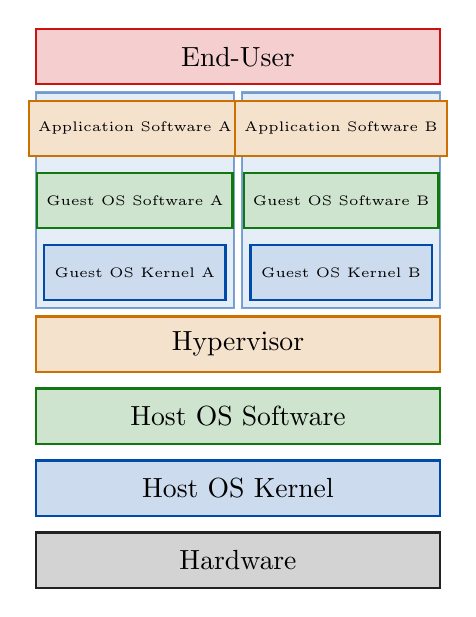
\begin{tikzpicture}[scale=1]
      \node[layer] at (\Center,\Height*1/2+\Sep*0) [draw=DarkGrey,fill=DarkGrey!20] {Hardware};
      \node[layer] at (\Center,\Height*3/2+\Sep*1) [draw=DarkBlue,fill=DarkBlue!20] {Host OS Kernel};
      \node[layer] at (\Center,\Height*5/2+\Sep*2) [draw=DarkGreen,fill=DarkGreen!20] {Host OS Software};
      \node[layer] at (\Center,\Height*7/2+\Sep*3) [draw=DarkOrange,fill=DarkOrange!20] {Hypervisor};
      \node[vmbox] at (\CenterL,\Height*11/2+\Sep*5) [draw=DarkBlue,fill=DarkBlue!20] {};
      \node[short] at (\CenterL,\Height*9/2+\Sep*4) [draw=DarkBlue,fill=DarkBlue!20] {\tiny Guest OS Kernel A \normalsize};
      \node[short] at (\CenterL,\Height*11/2+\Sep*5) [draw=DarkGreen,fill=DarkGreen!20] {\tiny Guest OS Software A \normalsize};
      \node[short] at (\CenterL,\Height*13/2+\Sep*6) [draw=DarkOrange,fill=DarkOrange!20] {\tiny Application Software A \normalsize};
      \node[vmbox] at (\CenterR,\Height*11/2+\Sep*5) [draw=DarkBlue,fill=DarkBlue!20] {};
      \node[short] at (\CenterR,\Height*9/2+\Sep*4) [draw=DarkBlue,fill=DarkBlue!20] {\tiny Guest OS Kernel B \normalsize};
      \node[short] at (\CenterR,\Height*11/2+\Sep*5) [draw=DarkGreen,fill=DarkGreen!20] {\tiny Guest OS Software B \normalsize};
      \node[short] at (\CenterR,\Height*13/2+\Sep*6) [draw=DarkOrange,fill=DarkOrange!20] {\tiny Application Software B \normalsize};
      \node[layer] at (\Center,\Height*15/2+\Sep*7) [draw=DarkRed,fill=DarkRed!20] {End-User};
   \end{tikzpicture}
\end{frame}

\begin{frame}\frametitle{Containers}
   \centering
   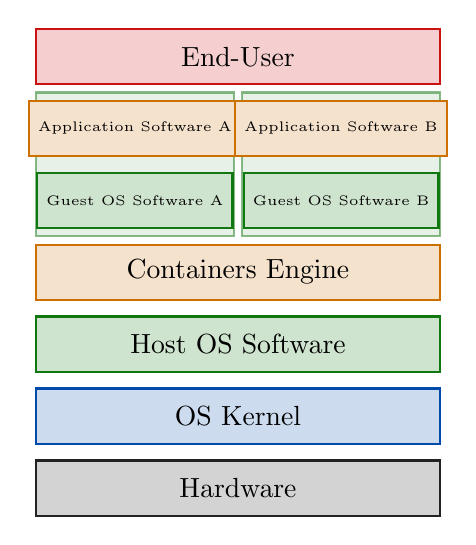
\begin{tikzpicture}[scale=1]
      \node[layer] at (\Center,\Height*1/2+\Sep*0) [draw=DarkGrey,fill=DarkGrey!20] {Hardware};
      \node[layer] at (\Center,\Height*3/2+\Sep*1) [draw=DarkBlue,fill=DarkBlue!20] {OS Kernel};
      \node[layer] at (\Center,\Height*5/2+\Sep*2) [draw=DarkGreen,fill=DarkGreen!20] {Host OS Software};
      \node[layer] at (\Center,\Height*7/2+\Sep*3) [draw=DarkOrange,fill=DarkOrange!20] {Containers Engine};
      \node[ctbox] at (\CenterL,\Height*5+\Sep*9/2) [draw=DarkGreen,fill=DarkGreen!20] {};
      \node[short] at (\CenterL,\Height*9/2+\Sep*4) [draw=DarkGreen,fill=DarkGreen!20] {\tiny Guest OS Software A \normalsize};
      \node[short] at (\CenterL,\Height*11/2+\Sep*5) [draw=DarkOrange,fill=DarkOrange!20] {\tiny Application Software A \normalsize};
      \node[ctbox] at (\CenterR,\Height*5+\Sep*9/2) [draw=DarkGreen,fill=DarkGreen!20] {};
      \node[short] at (\CenterR,\Height*9/2+\Sep*4) [draw=DarkGreen,fill=DarkGreen!20] {\tiny Guest OS Software B \normalsize};
      \node[short] at (\CenterR,\Height*11/2+\Sep*5) [draw=DarkOrange,fill=DarkOrange!20] {\tiny Application Software B \normalsize};
      \node[layer] at (\Center,\Height*13/2+\Sep*6) [draw=DarkRed,fill=DarkRed!20] {End-User};
   \end{tikzpicture}
\end{frame}

\begin{frame}\frametitle{Virtual Environments}
   \centering
   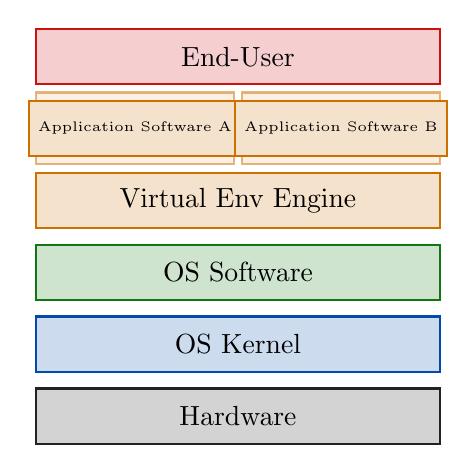
\begin{tikzpicture}[scale=1]
      \node[layer] at (\Center,\Height*1/2+\Sep*0) [draw=DarkGrey,fill=DarkGrey!20] {Hardware};
      \node[layer] at (\Center,\Height*3/2+\Sep*1) [draw=DarkBlue,fill=DarkBlue!20] {OS Kernel};
      \node[layer] at (\Center,\Height*5/2+\Sep*2) [draw=DarkGreen,fill=DarkGreen!20] {OS Software};
      \node[layer] at (\Center,\Height*7/2+\Sep*3) [draw=DarkOrange,fill=DarkOrange!20] {Virtual Env Engine};
      \node[vebox] at (\CenterL,\Height*9/2+\Sep*4) [draw=DarkOrange,fill=DarkOrange!20] {};
      \node[short] at (\CenterL,\Height*9/2+\Sep*4) [draw=DarkOrange,fill=DarkOrange!20] {\tiny Application Software A \normalsize};
      \node[vebox] at (\CenterR,\Height*9/2+\Sep*4) [draw=DarkOrange,fill=DarkOrange!20] {};
      \node[short] at (\CenterR,\Height*9/2+\Sep*4) [draw=DarkOrange,fill=DarkOrange!20] {\tiny Application Software B \normalsize};
      \node[layer] at (\Center,\Height*11/2+\Sep*5) [draw=DarkRed,fill=DarkRed!20] {End-User};
   \end{tikzpicture}
\end{frame}

\begin{frame}[fragile]\frametitle{Command Line Interpreter}
   \centering
   Like Linux,
   Python has a \\ [2ex]
   \Huge command line interpreter \normalsize \\ [2ex]
   \begin{lstlisting}[language=bash, style=bash, autogobble]
      (.v) $ python
      Python 3.8.5 (default, Jul 28 2020, 12:59:40)
      [GCC 9.3.0] on linux
      Type "help", "copyright", "credits" or "license" for more information.
      >>> 2+2
      4
      >>> print("Hello Python")
      Hello Python
      >>> import pathlib
      >>> pathlib.Path().absolute()
      PosixPath('/mnt/c/esilv/python')
      >>> print(_)
      /mnt/c/esilv/python
      >>>
   \end{lstlisting}
\end{frame}

\begin{frame}[fragile]\frametitle{Scripts}
   \centering
   Like Linux,
   Python allows to write \\ [2ex]
   \Huge scripts \normalsize \\ [2ex]
   \begin{lstlisting}[language=bash, style=bash, autogobble]
      (.v) $ cat pwd.py
      #!/usr/bin/env python3

      import pathlib

      current_path = pathlib.Path()
      print(current_path.absolute())

      (.v) $ python pwd.py
      /mnt/c/esilv/python
      (.v) $ ./pwd.py
      /mnt/c/esilv/python
      (.v) $ pwd
      /mnt/c/esilv/python
   \end{lstlisting}
   \vspace{2ex}
   \begin{center}
      Thanks to Shebang: \#!
   \end{center}
\end{frame}

%----------------------------------------------------------------------------------------
\subsection{Python Advantages}
%----------------------------------------------------------------------------------------

\begin{frame}[fragile]\frametitle{Modules}
   \centering
   Better than Linux,
   Python allows to write \\ [2ex]
   \Huge modules \normalsize \\
   that expose a Python Application Protocol Interface (\textbf{API}) \\ [2ex]
   \begin{lstlisting}[language=bash, style=bash, autogobble]
      (.v) $ cat mod.py
      import pathlib

      current_path=pathlib.Path()

      def pwd():
          print(current_path.absolute())

      (.v) $ python
      Python 3.8.5 (default, Jul 28 2020, 12:59:40)
      [GCC 9.3.0] on linux
      Type "help", "copyright", "credits" or "license" for more information.
      >>> import mod
      >>> mod.pwd()
      /mnt/c/esilv/python
      >>>
   \end{lstlisting}
   \vspace{1ex}
   \begin{center}
      With modules comes \textbf{Modularity} and \textbf{Higher Abstraction}
   \end{center}
\end{frame}

\begin{frame}[fragile]\frametitle{Modules CLI}
   \centering
   Modules can also expose a \textbf{CLI} \\ [1ex]
   \begin{lstlisting}[language=bash, style=bash, autogobble]
      (.v) $ cat setup.py
      import setuptools

      setuptools.setup(
          name='pypwd',
          entry_points={'console_scripts': ['pypwd = mod:pwd']},
      )
      (.v) $ pip install -e .
      Looking in indexes: https://pypi.org/simple
      Obtaining file:///mnt/c/esilv/python
      Installing collected packages: pypwd
        Running setup.py develop for pypwd
      Successfully installed pypwd
      (.v) $ pip list
      Package       Version Location
      ------------- ------- ----------------
      pip           20.0.2
      pkg-resources 0.0.0
      pypwd         0.0.0   /mnt/c/esilv/python
      setuptools    44.0.0
      (.v) $ pypwd
      /mnt/c/esilv/python
      (.v) $
   \end{lstlisting}
   \vspace{1ex}
   \begin{center}
      Thanks to Python entry points
   \end{center}
\end{frame}

% \begin{frame}\frametitle{GUI, CLI or API}
%    \begin{minipage}{0.55\linewidth}
%       \centering
%       \begin{tikzpicture}[scale=1]
%          \node[layer] at (\Center,\Height*1/2+\Sep*0) [draw=DarkGrey,fill=DarkGrey!20] {Hardware};
%          \node[layer] at (\Center,\Height*3/2+\Sep*1) [draw=DarkBlue,fill=DarkBlue!20] {OS Kernel};
%          \node[layer] at (\Center,\Height*5/2+\Sep*2) [draw=DarkGreen,fill=DarkGreen!20] {OS Software};
%          \node[layer] at (\Center,\Height*7/2+\Sep*3) [draw=DarkOrange,fill=DarkOrange!20] {Application Software};
%          \node[layer] at (\Center,\Height*9/2+\Sep*5) [draw=DarkRed,fill=DarkRed!20] {End User};
%          \visible<2->{
%          \draw[very thick, ->, >=stealth', DarkRed] (\Center*1/8,\Height*4+\Sep*5)
%                                                  -- (\Center*1/8,\Height*3+\Sep*2);
%          \node [DarkRed,below] at (\Center*1/8,\Height*3+\Sep*2) {\scriptsize GUI};
%          \draw[very thick, ->, >=stealth', DarkRed] (\Center*3/8,\Height*4+\Sep*5)
%                                                  -- (\Center*3/8,\Height*3+\Sep*2);
%          \node [DarkRed,below] at (\Center*3/8,\Height*3+\Sep*2) {\scriptsize CLI};}
%          \visible<3->{
%          \draw[very thick, ->, >=stealth', DarkRed] (\Center*7/8,\Height*4+\Sep*5)
%                                                  -- (\Center*7/8,\Height*4+\Sep*3);
%          \node [DarkRed,above left] at (\Center*7/8,\Height*4+\Sep*3) {\scriptsize GUI};
%          \draw[very thick, ->, >=stealth', DarkRed] (\Center*9/8,\Height*4+\Sep*5)
%                                                  -- (\Center*9/8,\Height*4+\Sep*3);
%          \node [DarkRed,above right] at (\Center*9/8,\Height*4+\Sep*3) {\scriptsize CLI};}
%          \visible<4->{
%          \draw[very thick, ->, >=stealth', DarkRed] (\Center*15/8,\Height*4+\Sep*5)
%                                                  -- (\Center*15/8,\Height*7/2+\Sep*3);
%          \node [DarkRed,below] at (\Center*15/8,\Height*7/2+\Sep*3) {\scriptsize API};}
%       \end{tikzpicture}
%    \end{minipage}
%    \begin{minipage}{0.41\linewidth}
%    \end{minipage}
% \end{frame}

% Survey:
% Which arrow(s) points to the shell ? 1, 2, 3, 4, 5 ? (1 and 2)

\begin{frame}\frametitle{Python vs Bash - choose the right tool}
   \centering
   You have a task to do: \\[2ex]
   \begin{itemize}
      \item Only once: GUI
      \item Several times: Bash
      \item With no Python interpreter: Bash
      \item That needs to run on Windows and Linux: Python
      \item That needs modularity, unit tests, debugging: Python
   \end{itemize}
\end{frame}

%----------------------------------------------------------------------------------------
\subsection{Python Useful Packages}
%----------------------------------------------------------------------------------------

\begin{frame}[allowframebreaks]\frametitle{Python Standard Library Extract}
   \begin{itemize}
      \item Data Types and Data Structures:
      \begin{itemize}
         \item \textcolor{DarkBlue}{datetime} - Basic date and time types
         \item \textcolor{DarkBlue}{math} - Mathematical functions
         \item \textcolor{DarkBlue}{enum} - Support for enumerations
         \item \textcolor{DarkBlue}{collections} - Container datatypes
         \item \textcolor{DarkBlue}{queue} - A synchronized queue class
         \item \textcolor{DarkBlue}{itertools} - Functions creating iterators for efficient looping
      \end{itemize}
      \vspace{0.3em}

      \item Text and Files:
      \begin{itemize}
         \item \textcolor{DarkBlue}{json} - JSON encoder and decoder
         \item \textcolor{DarkBlue}{csv} - CSV File Reading and Writing
         \item \textcolor{DarkBlue}{glob} - Unix style pathname pattern expansion
         \item \textcolor{DarkBlue}{re} - Regular expression operations
         \item \textcolor{DarkBlue}{pathlib} - Object-oriented filesystem paths
         \item \textcolor{DarkBlue}{difflib} - Helpers for computing deltas
         \item \textcolor{DarkBlue}{filecmp} - File and Directory Comparisons
         \item \textcolor{DarkBlue}{tempfile} - Generate temporary files and directories
      \end{itemize}
      \vspace{0.3em}

      \item Algorithms:
      \begin{itemize}
         \item \textcolor{DarkBlue}{copy} - Shallow and deep copy operations
         \item \textcolor{DarkBlue}{random} - Generate pseudo-random numbers
         \item \textcolor{DarkBlue}{hashlib} - Secure hashes and message digests
         \item \textcolor{DarkBlue}{zlib} - Compression compatible with gzip
      \end{itemize}
      \vspace{0.3em}

      \item Integration:
      \begin{itemize}
         \item \textcolor{DarkBlue}{argparse} - Parser for command-line options, arguments and sub-commands
         \item \textcolor{DarkBlue}{logging} - Logging facility for Python
         \item \textcolor{DarkBlue}{subprocess} - Subprocess management
         \item \textcolor{DarkBlue}{timeit} - Measure execution time of small code snippets
         \item \textcolor{DarkBlue}{sys} - System-specific parameters and functions
         \item \textcolor{DarkBlue}{os} - Miscellaneous operating system interfaces
      \end{itemize}
   \end{itemize}
\end{frame}

\begin{frame}[allowframebreaks]\frametitle{Python Third-party Packages Extract}
   \begin{itemize}
      \item Image and Video Processing:
      \begin{itemize}
         \item \textcolor{DarkBlue}{Pillow} - Image Processing
         \item \textcolor{DarkBlue}{OpenCV} - Computer vision
         \item \textcolor{DarkBlue}{Moviepy} - Movie editing
      \end{itemize}
      \vspace{0.3em}

      \item Web:
      \begin{itemize}
         \item \textcolor{DarkBlue}{Requests} - HTTP requests more responsive and user-friendly
         \item \textcolor{DarkBlue}{Selenium} - Web browser automaton
         \item \textcolor{DarkBlue}{Scrapy} - Web crawler
         \item \textcolor{DarkBlue}{BeautifulSoup} - HTML and XML parser
         \item \textcolor{DarkBlue}{Django} - Web Framework
         \item \textcolor{DarkBlue}{Flask} - Micro Web Framework
      \end{itemize}

      \item Machine Learning:
      \begin{itemize}
         \item \textcolor{DarkBlue}{Keras} - Deep neural networks
         \item \textcolor{DarkBlue}{TensorFlow} - ML, Dataflow and Differentiable Programming
         \item \textcolor{DarkBlue}{Scikit Learn} - Machine Learning
         \item \textcolor{DarkBlue}{PyTorch} - Machine Learning
      \end{itemize}
      \vspace{0.3em}

      \item Scientific Calculus and Data Science:
      \begin{itemize}
         \item \textcolor{DarkBlue}{Numpy} - N-dimensional array processing
         \item \textcolor{DarkBlue}{Pandas} - Data Analysis and Dataframes
         \item \textcolor{DarkBlue}{Scipy} - Scientific and technical computation
         \item \textcolor{DarkBlue}{Matplotlib} - Data Visualization 2-dimensional graphs and plots
         \item \textcolor{DarkBlue}{Bokeh} - HTML and JavaScript Data Visualization
      \end{itemize}
      \vspace{0.3em}

      \item Software Engineering:
      \begin{itemize}
         \item \textcolor{DarkBlue}{SQLAlchemy} - Database Abstraction
         \item \textcolor{DarkBlue}{PyMongo} - Interact with MongoDB database
         \item \textcolor{DarkBlue}{Fire} - Automatically generate CLI (command-line interface)
         \item \textcolor{DarkBlue}{Pytest} - Unit tests
         \item \textcolor{DarkBlue}{Fabric} - Software Deployment
         \item \textcolor{DarkBlue}{Supervisor} - Services controller
      \end{itemize}
      \vspace{0.3em}

      \item Specific Formats Processing:
      \begin{itemize}
         \item \textcolor{DarkBlue}{XlsxWriter} - Excel .xlsx files creator
         \item \textcolor{DarkBlue}{PyYAML} - YAML implementations for Python
         \item \textcolor{DarkBlue}{PyPDF2} - PDF split, merge and transform
      \end{itemize}
      \vspace{0.3em}

   \end{itemize}
\end{frame}

%----------------------------------------------------------------------------------------

\end{document}
